\documentclass[12pt, a4paper]{article}
\usepackage[utf8]{inputenc}
\usepackage[russian]{babel}
\usepackage[T2A]{fontenc}
\usepackage{amsfonts}
\usepackage{amsmath}
\usepackage{indentfirst}
\usepackage{amsthm}
\DeclareMathOperator*{\argmin}{argmin}
\newtheorem{lemma}{Лемма}[section]

\usepackage[left=2cm,right=1.5cm,top=2cm,bottom=2cm]{geometry}
\linespread{1.25}

\usepackage{graphicx}
\graphicspath{{pictures/}}
\DeclareGraphicsExtensions{.pdf,.png,.jpg}

\begin{document}
 \section*{Тема}
Построение оптимального маршрута при заданной модели движения других участников транспортной сети


\section{Введение}

В данной работе рассматривается задача нахождения наилучшего в каком-то смысле пути с учетом движения фиксированного количества участников по заданным ранее маршрутам в условиях ограниченности модели дорожной системы. Новый построенный маршрут должен отвечать выбранным критериям кратчайшести среди всевозможных путей на всем временном промежутке, но не обязательно в каждый момент времени. Знание маршрутов изначальных участников помогает определить плотность автомобильного потока на конкретных отрезках пути. Рассматриваемая модель приближена к реальной дорожной системе городов, поэтому на всех ее участках наложены ограничения по вместимости участников и скорости их движения. Такие ограничения влияют на показатели маршрутов участников, такие как итоговое время движения и длину пути. 


Тема актуальна в наше время, так как она помогает решить проблему пробок на дорогах, а также призвана упростить водителям выбор маршрута, который займет у них наименьшее время. Задача имеет практический характер... Проблема пробок в Москве стоит очень остро, ученые решают ее не первый год..

В мире прогнозы загруженности используются для автоматического управления дорожным движением в некоторых городах. Первые прототипы, в которых были применены прогнозы, появились появились в 1998 году в США. А первое пилотное использование системы, «заглядывающей в будущее», началось в 2006 году в Сингапуре. Среди наших соотечественников похожей задачей занимается отдел навигации Яндекса. Разработчики собирают информацию по трекам движения автомобилей, осуществляют привязку треков к ребрам графа дорожной сети, вычисляют некоторую усредненную скорость на отдельных участках, рисуют карту прогноза дорожной ситуации на ближайший час и в связи с этим предлагают оптимальный по времени путь, а также еще пару алтернативных маршрутов. Сложность сбора информации и построения треков движения состоит в том, что, во-первых, не все пользуются сервисами Яндекса при построении своего маршрута, и во-вторых, в данных постоянно возникают лишние шумы, что приводит к выбросам на графиках, и с таким качеством информации работать очень сложно. Мы же рассматриваем более прозрачную и простую модель, когда все маршруты изначально проложены и нам известны, и они не меняются с течением времени. Это не умаляет значимости и важности поставленной нами задачи. Мы получим более четкие результаты, идеи в дальнейшем могут развиваться и открывать новые возможности для более широкой задачи, например, как у Яндекса. Также стоит отметить, что специалисты по навигации используют статистические методы и машинное обучение в качестве инструмента для решения своих задач, мы же подойдем к вопросу с другой стороны и применим другие алгоритмы. На данный момент отдел навигации Яндекса проводит улчшения своих методов и подходов к решению задач, а также придумывает какие-то новые метрики и способы оценки качества этих решений.


Задачи, которые мы ставили перед собой в рамках выбранной темы дипломной работы: формальная постановка задачи, анализ полученных ранее результатов в этой теме, разработка простого алгоритма решения на основе моделирования и его оценка, оценка устойчивости полученного решения, попытка обощения дорожной сети, ее расширение (или сужение?). Методы исследования включают в себя: построение графа с вершинами в концевых точках заданных маршрутов и ребрами, отображающими дороги между ними, определение функции веса-загруженности дорог, 



Основа нашей задачи - нахождение наилучшего пути в условиях изменчивости плотности и скорости дорожного потока на участках в заисимости от времени.

В первой главе вы сможете ознакомиться с деталями поставленной задачи, далее мы решим ее путем моделирования дорожной ситуации и применением некоторых известных алгоритмов, в третьей главе поговорим о достоинствах и недостатках такого решения, его сложности и реализуемости в реальной жизни. Четвертая глава будет содержать описание некоторых модификаций графа дорожной сети, а также улучшений решения на таком графе. В завершении поделимся результатами проделанной работы, оценим их качество и сделаем выводы.




\newpage
\section{Постановка задачи}
Пусть задан ориентированный \textit{граф дорожной сети} $ G (V, E, l)$ таким образом, что вершины $ v \in V$ осуществляют роль перекрестков, а ребра $e \in E$ - роль дорог. Каждое ребро имеет длину, т.е. задана функция $l : E \rightarrow \mathbb {R} $. Также задана \textit{система правил} движения АТС -- набор неравенств, определяющих поведение участников в каждый момент времени.

Пусть имеется $n$ участников, которые движутся по заранее заданным маршрутам:  $ p_i = \langle E^i_{j_1}, E^i_{j_2}, \dots, E^i_{j_{m_i}} \rangle$, $ E^i_{j_k} \in E \quad i = 1, \dots, n$. И к ним добавляется $(n+1)$-ый участник, которому нужно добраться из пункта $A$ в пункт $B$, $A, B \in V$. Определим $P(A,B)$~-- множество всех простых путей из $A$ в $B$. Правила движения позволяют определить \textit{часть пройденного пути} для каждой АТС в зависимости от движения других участников, т.е. определить непрерывные функции
\begin{center}
 $x^{p_i}_i(G, \cdot ) : \mathbb {R} \rightarrow [0 , 1] $, $i = 1, \dots, n$ \\ $x^{p}_{n+1}(G, \cdot ) : \mathbb {R} \rightarrow [0 , 1]$, $p \in P(A, B) $.
\end{center}
Ввиду однозначной определенности последовательности ребер, по которым осуществляется движение, индекс, означающий путь $p_i$, для заданных $n$ участников можно опустить. Также для простоты записи не будем писать зависмость функций от графа $G$. Считаем, что первые $n$ участников влияют на движение всех АТС, но их движение не зависит от $(n+1)$-ого добавленного участника. Будем говорить, что функции 
\begin{center}
	$x_i(t) : \mathbb {R} \rightarrow [0 , 1] $, $i = 1, \dots, n$ \\ $x^{p}_{n+1}(t) : \mathbb {R} \rightarrow [0 , 1]$, $p \in P(A, B) $.
\end{center}
\textit{задают модель движения} АТС.

На множестве путей $P(A,B)$ определим $T(p) = \displaystyle \inf_t \{t : x^p_{n+1}(t) = 1\}$~-- время прибытия $(n+1)$-ого участника в вершину $B$ при движении по маршруту $p$. Требуется найти такой путь $p^* \in P(A, B)$, что $T(x^{p^*}_{n+1})$ - минимальна. Другими словами, на графе $G(V, E, l)$ при движении $n$ участников по фиксированным путям для заданных вершин $A$ и $B$ требуется найти путь
$$p^* = \argmin_{p \in P(A, B)} T(x^p_{n+1}).$$

\newpage
\section{Возможные правила движения}

Нас интересует точное решение, поэтому промоделируем движение $n$ участников, чтобы в каждый момент времени были известны функции $x_i(t)$. Для этого сначала зададим правила движения АТС на графе $G(V, E, l)$.

Опишем модель \textit{следования за лидером}~-- модель, в которой поведение движения участника зависит от взаимодействия с впереди идущим АТС. Определим функции \textit{скорости} $v_i(t) = \dot{x}_i(t)$ и \textit{ускорения} $a_i(t) = \dot{v}_i(t) = \ddot{x}_i(t)$. Обозначим через $v_m \in \mathbb {R}$ максимально возможную скорость, или \textit{скорость свободного движения}: $v_i(t) \leq v_m, \forall t \in \mathbb {R}, i = 1, \dots, n$. Введем также \textit{безопасное расстояние} $D$~-- дистанция, на котором участники  характер движения лидера  

\begin{enumerate}
	\item 
	
\end{enumerate}


\newpage
\section{Решения}

Первое, что приходит на ум в качестве решения, это перебор всех возможных путей и нахождение подходящего по затраченному времени. Посчитаем сложность этого алгоритма и сделаем вывод о его использовании в нашей задаче на практике.

\subsection{Перебор. Сложность}
Чтобы узнать, применим ли перебор в нашем случае, посчитаем сложность нахождения кратчайшего пути среди множества всех простых путей из $A$ в $B$. Пусть $S_x(p)$~-- сложность нахождения функции $x^p_{n+1}(t)$, при выборе пути $p$. Тогда сложность перебора
\begin{center}
 $S = \sum\limits_{p \in P(A,B)} S_x(p) = \vert P(A,B) \vert * \overline S_x$, где $\overline S_x$~-- средняя сложность.
\end{center}
Заметим, что $ S $ растет при увеличении количества возможных путей. Так, в полном графе на $\vert V \vert$ вершинах получим $S = 2^{|V|-2} * \overline S_x$.

В качестве примера можем рассмотерть также регулярный граф-решетку на $\mathbb {R}^2$ и на нем оценить снизу сложность поиска пути с минимальными тратами. Пусть точки $A$ и $B$ имеют координаты $(a_1, a_2)$ и $(b_1, b_2)$ соответственно. Тогда количество путей минимальной длины в метрике Манхэтенна будет составлять $C^{|a_1-b_1|}_{|a_1-b_1| + |a_2-b_2|}$. Понятно, что путей $|P(A,B)|$ в таком графе гораздо больше. Таким образом, получаем оценку снизу для регулярного решеточного графа

\begin{center}
	$C^{|a_1-b_1|}_{|a_1-b_1| + |a_2-b_2|} * \overline S_x  \leq  \vert P(A,B) \vert * \overline S_x = S$.
\end{center}

Например, в решетке-квадрате со стороной $m$ при движении из угловой точки по диагонали в угловую точку напротив количество путей минимальной длины составит $C^m_{2m} = \frac{(2m)!}{m!m!} $. По формуле Стирлинга
\begin{center}
 $ C^m_{2m} = \frac{\sqrt{2\pi(2m)} \left( \frac{2m}{\exp} \right)^{2m}}{\left(\sqrt{2\pi m} \left( \frac{m}{\exp} \right)^m \right)  \left(\sqrt{2\pi m} \left( \frac{m}{\exp} \right)^m \right)} = \frac{2\sqrt{\pi m} \left( \frac{2m}{\exp} \right)^{2m}}{2\pi m \left( \frac{m}{\exp} \right)^{2m}} = \frac{2^{2m}}{\sqrt{\pi m}}$.
\end{center}
Понятно, что при увеличении $m$, количество путей экспоненциально растет.

С помощью перебора можно находить кратчайшие пути быстро, если $|P(A,B)|$ не велико. Однако изначально наша задача была сформулирована в терминах дорожной сети и предполагала графы с достаточно большим количеством вершин и ребер, что влияет на количество маршрутов для заданных точек. Таким образом, можно сделать вывод, что в общем случае перебор путей в нашей задаче на практике не применим.

\newpage
\subsection{Дейкстра}


Рассмотрим вспомогательную задачу. Пусть на каждом ребре $e \in E$ графа $G(V, E)$ определена функция \textit{временных затрат} $\phi_e(t) : \mathbb {R}_+ \rightarrow \mathbb {R}_+$. Если мы оказались в начальной вершине ребра $e$ в момент времени $t$, то время преодоления ребра будет равняться $\phi_e(t)$. Рассмотрим путь $p = \langle V_0, e_1, V_1, e_2, V_2, \dots, V_{k-1}, e_k, V_k \rangle $ и начало движения происходит в вершине $V_0$ в момент времени $t_0 = t$, тогда
\begin{align*}
t_0 & = t  \\
t_1 & = \phi_{e_1}(t) + t = \phi_{e_1}(t_0) + t_0  \\
t_2 & = \phi_{e_2}(\phi_{e_1}(t) + t) + \phi_{e_1}(t) + t = \phi_{e_2}(t_1) + t_1 \\
    & \dots \\
t_i & = \phi_{e_i}(t_{i-1}) + t_{i-1} \\
    & \dots \\
t_k & = \phi_{e_k}(t_{k-1}) + t_{k-1}
\end{align*}
Пусть $P(A, B)$~-- множество всех простых путей из $A$ в $B$ в графе $G(V, E)$. Необходимо найти путь из $A$ в $B$, который требует минимальных затрат, т.е. 
\begin{center}
$\begin{cases}
	t_{|p|} \rightarrow min \\
	p \in P(A, B)
\end{cases}$
\end{center}
В общем случае функции временных затрат могут быть любыми. Давайте рассмотрим эту задачу с дополнительным условием на $\phi_e(t):$
$$ \phi_e(t) \leq \Delta + \phi_e(t + \Delta), \quad \Delta \ge 0$$
Назовем это условие \textit{неравенством прохождения ребер}. Утверждается, что если для $\forall e \in E$ функции временных затрат $\phi_e$ удовлетворяют неравенству прохождения ребер, то задачу можно решить модифицированным алгоритмом Дейкстры.

\subsubsection{Модифицированный алгоритм Дейкстры}
%\newpage
%\section*{Алгоритм Дейкстры}

%$\textbf{Неравенство прохождения ребер}$

%Будем считать, что наша дорожная сеть обладает условием FIFO : чем позже въехать на дорогу, тем позже получится ее преодолеть (?).\\
%Перенесем это на математический язык : \\
%Пусть время прохождения по ребру задается формулой $f(t)$, где $t$ - время старта. Тогда получим, что $f(t) \le \Delta + f(t + \Delta)$, при $\Delta \ge 0$. Назовем это \textit{неравенством прохождения ребер}.


$\textbf{Алгоритм построения минимального маршрута}$

Для каждой вершины будем хранить два значения: минимальное время, за которое можно добраться до этой вершины, и ребро, через которое проходит кратчайший маршрут до вершины.
%Если вес для ребра из вершины задается формулой $f(t)$,а минимальное время для этой вершины -- $x$, то за текущий вес ребра будем брать $f(x)$.
Применяем стандартный алгоритм Дейкстры, с отличием, что при посещении вершины мы фиксируем время для нее и пересчитываем функции временных затрат на всех ребрах, исходящих из этой вершины.\\
Для запуска алгоритма потребуется задать начальное время - минимальное время в точке старта. Это можно использовать в анализе маршрута.


\begin{lemma}
Данный маршрут обладает наименьшим временем прохождения.
\end{lemma}

\begin{proof}

Будем доказывать по индукции :\\
База индукции - в графе 2 вершины и несколько ребер между ними. Минимальным маршрутом будет то ребро, у которого наименьшее время прохождения.\\
Шаг индукции - считаем что в случае с m (< n) вершинами лемма справедлива. Рассмотрим граф, содержащий n вершин. Пусть $\exists$ маршрут P в этом графе, требующий меньше затрат, чем построенный нашим алгоритмом, тогда возьмем ближайшую к началу точку, обозначим ее $C$, в которой выбрано ребро, отличное от минимального по затратам. Очевидно, что если точка $C$ совпадает с точкой $F$, концом маршрута, то P не является минимальным по времени прохождения. \\
Пусть ребро маршрута P в точку $C$ выходит из точки $B$, а минимальное - из точки $A$. Построим маршрут по нашему алгоритму из $S$ -- начала маршрута в $C$. Заметим, что он проходит через точку $A$. Обозначим время этого маршрута за $t_a = T(S-...-A-C)$, а время для части маршрута P из $S$ в $C$, проходящего через точку $B$, за $t_b = T(S-...-B-C)$. В подграфе $(P-C)$ вершин меньше чем $n$, а значит по индукции $t_a$ < $t_b$. 
\begin{center}
	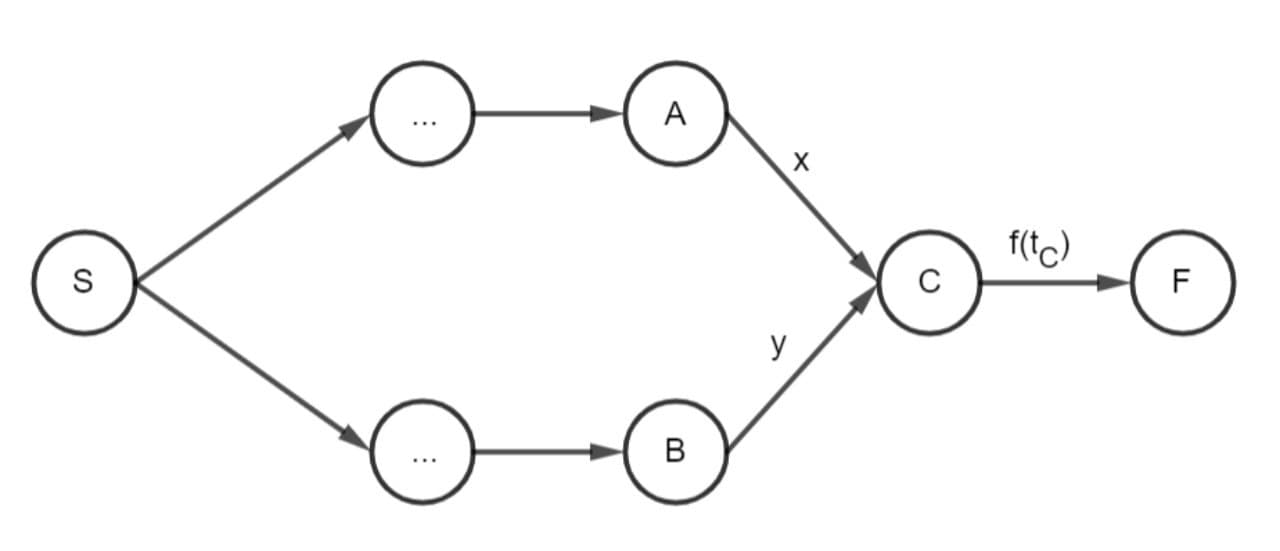
\includegraphics[scale=0.3]{graph_1.jpg}
\end{center}

Без ограничения общности, будем рассматривать часть маршрута P от точки C до F как одно ребро : C-F. Тогда время прохождения этого ребра $\phi(t_C) = \phi_{CF}(t_C)$, где $t_C$ - время старта из точки $C$. Вспомним неравенство прохождения для ребер (см. выше) : $\phi(t_a) \le (t_b - t_a) + \phi(t_b)$, где $\Delta = (t_b - t_a)$

Рассмотрим два маршрута $P : S-...-B-C-F$ и $P': S-...-A-C-F$.
Посчитаем время : $T(P) = t_b + \phi(t_b)$  и $T(P') = t_a + \phi(t_a)$
Используя неравенство, получаем : $T(P') = t_a + \phi(t_a) \le t_a + (t_b - t_a) + \phi(t_b) = T(P)$ Значит маршрут P не является минимальным.

\end{proof}

Понятно, что если неравенство прохождения ребер не выполняется, то модифицированный алгоритм Дейкстры может построить не кратчайший маршрут в терминах временных затрат. Рассмотрим такой пример (рис. 1):
\begin{align*}
	p_1: & \\
	& t_0 = 0 \\
	& \phi_{AC}(t) = 1  \\
	& \phi_{CB}(t) = 1 + 2 * \mathbb{I} \{t < 1.5\} \\
	p_2: & \\
	& t_0 = 0 \\
	& \phi_{AC}(t) = 2  \\
	& \phi_{CB}(t) = 1 + 2 * \mathbb{I} \{t < 1.5\} 
\end{align*}
Время прохождения пути $p_1$ будет составлять $t_{p_1} = t_0 + \phi_{AC}(t_0) + \phi_{CB}(\phi_{AC}(t_0)) = 1 + 3 = 4 $. Время прохождения пути $p_2$ будет составлять $t_{p_2} = 1 + 1 = 2 $. Очевидно, на путь $p_2$ потребуется меньше времени, чем на путь $p_1$, но алгоритм Дейкстры предложит в качестве решения задачи маршрут $p_1$.

\begin{figure}[!hbp]
	\centering
		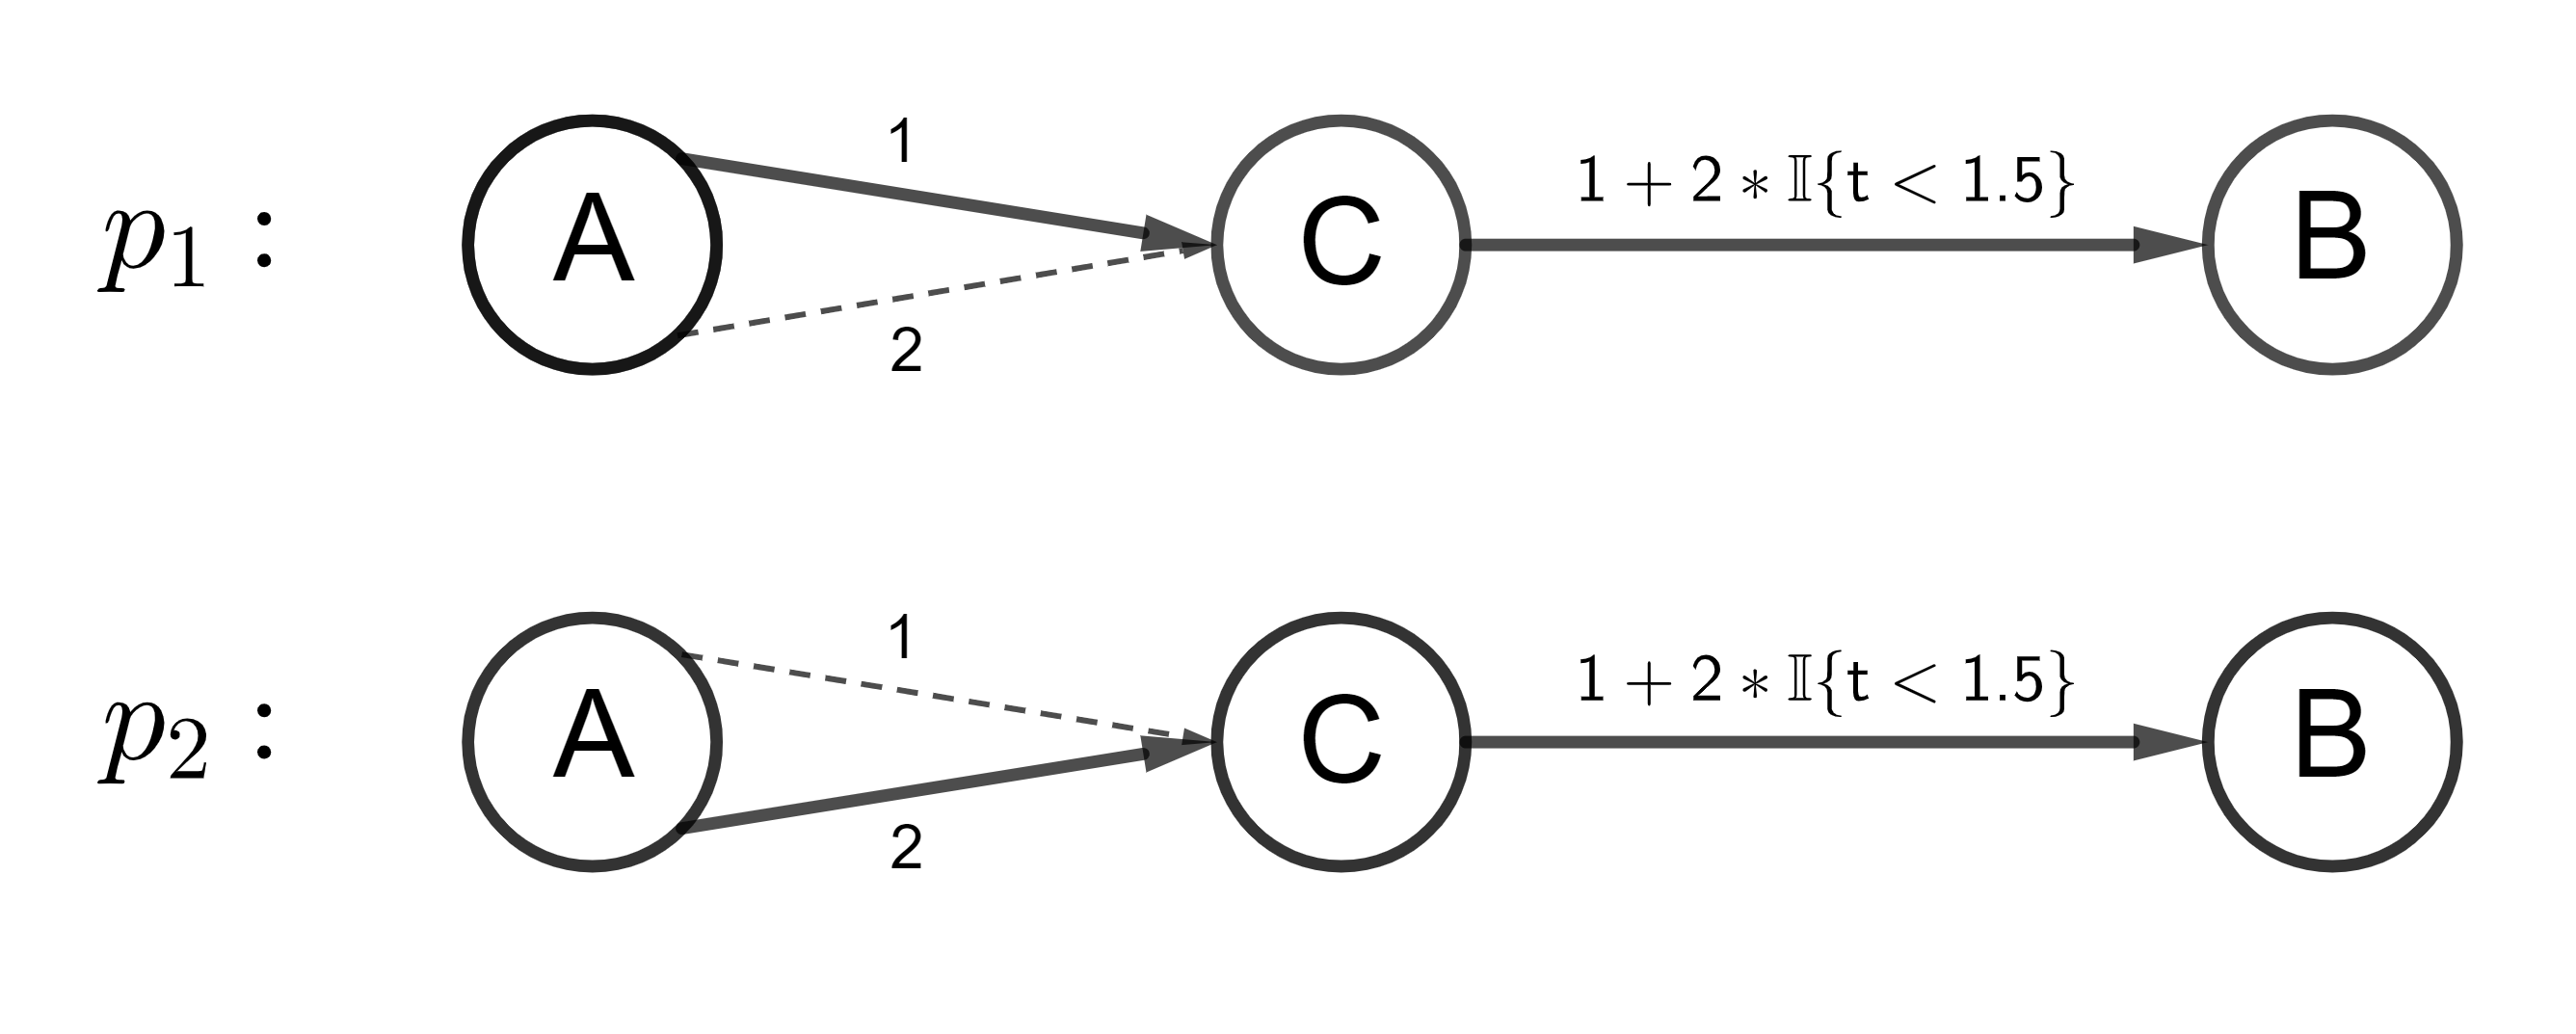
\includegraphics[scale=0.2]{graph_2.png}
	\caption{Пример графа с невыполненным условием неравенства прохождения ребер}
\end{figure}




\newpage
\section*{Устойчивость нашего решения}



\newpage
\section*{Практические результаты}


\newpage
\section*{Сложность решения}

\newpage
\section*{Альтернативные подходы}

\newpage
\section*{Заключение}

\newpage
\section*{Список литературы}

\end{document}